\documentclass[a4paper,12pt]{article}

\usepackage{graphicx} % For including images
\usepackage{longtable} % For tables that span multiple pages
\usepackage{multirow} % Formultirow command for tables
\usepackage{wrapfig}
\usepackage{fancyhdr}
\usepackage[l3]{csvsimple}  % For importing CSV data
\usepackage{subfig}



\pagestyle{fancy}
\fancyhf{}
\fancyhead[L]{
\includegraphics[height=1cm]{iitblogo.png}}  % Adjust the height as needed
\fancyhead[R]{\textbf{INDIAN INSTITUTE OF TECHNOLOGY} \\ \textbf{Powai , Mumbai , 492006}}                     % Your text

\begin{document}


\vspace{1cm} % Adjust spacing as needed
\begin{tabular}{p{5cm}p{7cm}}
  \textbf{Roll Number} &\csvreader[
  head=true,
  tabular = c
  ]{
  student.csv
  }{}{\csvcoli} \\
  \textbf{Date of Issue}  & $10^{th}$ May 2024 \\
  \textbf{Name of the Student} &\csvreader[tabular = c]{student.csv}{}{\csvcolii} \\
  \textbf{Programme}  & Bachelor of Technology (B.Tech.) \\
\end{tabular}

\vspace{0.25cm} % Adjust spacing as needed

\begin{center}
  \textbf{Transcript}
\end{center}
\centering
 \csvautotabular{student.csv}

\section*{Statistics}
\csvautotabular{stats.csv}
% \textbf{Signature & Seal of Transcript Issuing Authority}
\vspace{0.5cm}
\section*{Performance Analysis}
\begin{figure}[bh]
    \centering
    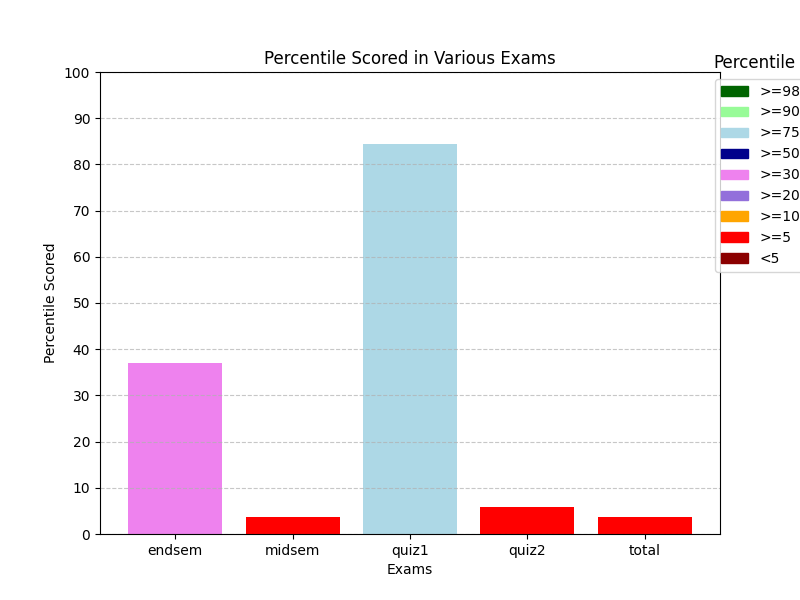
\includegraphics[width=0.7\textwidth]{barGraph.png}
    \caption{Bar Graph Depicting the Percentile}
\end{figure}

\newpage

\begin{figure}[th]
    \centering
    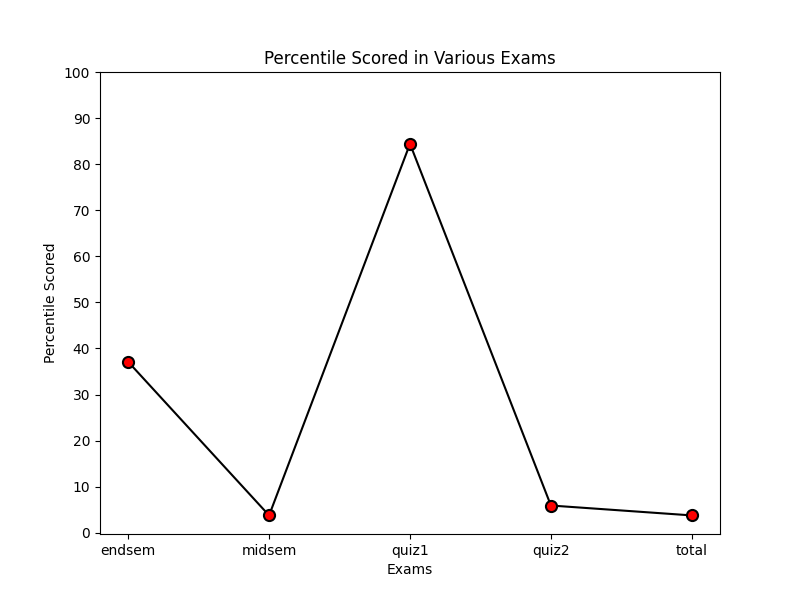
\includegraphics[width=0.7\textwidth]{lineGraph.png}
    \caption{Line graph Depiciting the Percentile through out various exams}
\end{figure}

\section*{Grades}
    \textit{}{\Large Your Grade in This Subject is \textbf{\input{gradeStudent.txt}}}

\section*{Remarks}
\begin{itemize}
   \item \input{exam-wise-remarks.txt}
   \item \input{Overall.txt}
\end{itemize}

\end{document}